%不需修改部分
\documentclass[UTF8]{ctexart}  %使用中文版的article文档类型排版,并选择UTF8编码格式
\usepackage{algorithm}
\usepackage{algorithmic}
\usepackage{amsmath}
\usepackage[colorlinks,linkcolor=black,anchorcolor=blue,citecolor=green]{hyperref}    %修改特定内容的颜色
\usepackage{enumerate}                      %条目包
\usepackage{float}                          %固定表格位置
\usepackage{graphicx}                       %图片包
\usepackage{float}                          %设置图片浮动位置的宏包
\usepackage{subfigure}                      %插入多图时用子图显示的宏包
\usepackage{titlesec}                       %自定义多级标题格式的宏包
\usepackage{geometry}
\usepackage{wrapfig}
\pagestyle{plain}						    %显示页码
\RequirePackage{fix-cm}                     
\usepackage{longtable}
\usepackage{listings}
\usepackage{setspace}
\usepackage{xcolor}
\usepackage{caption}
\usepackage{diagbox}
\usepackage{multirow} %合并多行单元格的宏包
\usepackage{longtable} %不宽但很长的表格可以用longtable宏包来进行分页显示
\usepackage{array} %一般用于数学公式中对数组或矩阵的排版
\usepackage{makecell}% makecell命令对表格单元格中的数据进行一些变换的控制。我们可以使用 \ 命令进行换行,也可以使用p{(宽度)}选项控制列表的宽度
\usepackage{threeparttable} %制作三线表格
\usepackage{booktabs}%s三线表格中的上中下直线线型设置宏包,在这个包中水平线被教程\toprule、midrule、buttomrule。

%标题格式,可根据需要进行修改
\titleformat{\section}[block]{\Large\bfseries}{\arabic{section}.}{1em}{}[]
\titleformat{\subsection}[block]{\large\itshape\bfseries}{\arabic{section}.\arabic{subsection}}{1em}{}[]
\titleformat{\subsubsection}[block]{\normalsize\bfseries}{\arabic{section}.\arabic{subsection}.\arabic{subsubsection}}{1em}{}[]
\titleformat{\paragraph}[block]{\small\bfseries}{[\arabic{paragraph}]}{1em}{}[]

\geometry{a4paper,left=2cm,right=2cm,top=2cm,bottom=2cm}



\begin{document}

\begin{titlepage} %制作封面
        \heiti
        \vspace*{100pt}
        \begin{center}
            \fontsize{48pt}{0} 人\quad 工\quad 智\quad 能\quad 导\quad 论\\
            \vspace*{36pt}
            \fontsize{36pt}{0}{第\quad 二\quad 次\quad 大\quad 作\quad 业\quad 实\quad 验\quad 报\quad 告}\\
            \vspace*{48pt}
            \LARGE(2023\ -\ 2024\ 学年度\qquad 春季学期)\\
            \vspace*{48pt}

            \LARGE 实验名称\ \ \underline{\makebox[300pt]{智能车运送货物}}\\
            \vspace*{72pt}

            \heiti\Large 姓名\ \ \underline{\makebox[168pt]{\songti 张章}}\\
            \heiti\Large 学号\ \ \underline{\makebox[168pt]{\songti 2023010916}}\\
            \heiti\Large 院系\ \ \underline{\makebox[168pt]{\songti 自动化系}}\\
            \heiti\Large 教师\ \ \underline{\makebox[168pt]{\songti 张长水}}\\
			\heiti\Large 时间\ \ \underline{\makebox[168pt]{\songti 2024/5}}\\
        \end{center}
\end{titlepage}

\tableofcontents %插入目录
\thispagestyle{empty}

\newpage %正文
\section{摘要}
本实验旨在设计一种算法完成对多智能体的路径规划,使得各个智能体能够无冲突地完成将货物从一个仓库转移至另一个仓库的
任务。在本实验中,作者设计了一种方法将该问题转换成一系列经典的多智能体路径规划问题,并使用基于冲突的搜索算法解决
这一系列的多智能体规划问题。实验结果和项目仓库已经上传至Githuhb,请通过以下链接查看:




\section{相关工作}
\section{定义实验任务}
大作业的作业题目并没有对本次实验要完成的内容做出详细的指示,因此在介绍实验方法前,作者将先对实验任务进行定义。

本次实验中,我们将随机生成一幅地图,地图上分布着由等大的小正方形组成的障碍物以及仓库$A$和仓库$B$。我们假设在初始
状态下在仓库$A$存在着$N$件货物。$M$辆无人货车随机地分布在地图上的各处,它们在单位时间内能够向上下左右四个方向移动
的距离固定,每辆货车最多只能装载一个货物。考虑到实际情况,我们认为$M$应当小于$N$。因此,我们的任务可以定义为,规划
所有小车的路线,使它们在两个仓库之间来回折返,运送货物,直到所有的货物都移动至$B$仓库为止。且这些货车的路线应当满足:
1)小车路线要能自主避开障碍物;2)这些路线两两之间并无冲突,即两辆货车不会在同一时间占据同一个位置,也不会在某一时刻
彼此交换位置,如图1所示;3)在满足前两个条件的前提下,路径花费的代价应该尽可能少,也就是所有小车移动距离的总和最小。

在实现对所有货车路径的规划之后,我们还需要使用可视化的方法展示。


\begin{figure}[H]
    \centering
    \centering
    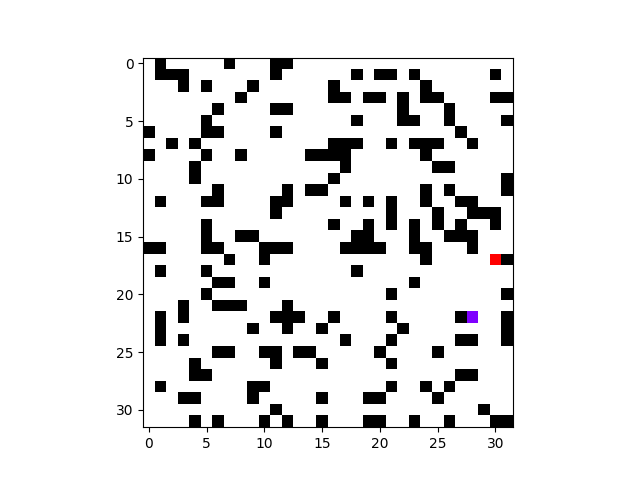
\includegraphics[width=0.6\textwidth, keepaspectratio]{fig1.png}
    \captionsetup{font=footnotesize}
    \caption{图中展示了两种冲突的可能,左侧表示两小车在同一时刻占据同一位置,右侧表示两小车在某一时刻互换位置}
    \label{figure1}
\end{figure}



\section{实验目标}
\section{实验方法}
本次实验中,作者将本次实验的任务分解成一系列经典的多智能体路径规划(Multiple Agent Path Finding, 以下简称MAPF)问题,
然后使用基于冲突的搜索(Conflicts-Based Search, 以下简称CBS)算法解决这些MAPF问题,最终得到整个问题的解。CBS的底层寻路
算法,作者使用了时空联合A*算法。
\subsection{全局算法}
单个小车的状态和仓库A状态的组合有下述四种情况:1)小车没货,仓库A有货 2)小车有货,仓库A有货 3)小车有货,仓库A没货 4)小车没货,仓库A没货
上述四种情况对应小车的三种任务:1)从当前位置去仓库A取货 2)从当前位置去仓库B送货 3与4)从当前位置前往所有小车的集合点
如果小车有货,就要去B,如果没货再判断,如果此时
所有小车记作$\bf c$,在某一时刻$t_0$,所有的小车的状态记作$\bf x_n$,所有小车完成当前任务之后的状态记作$\bf x_{n+1}$(此时我们假设先到达目标位置的小车在到达之后暂停运动),可以发现,从$\bf x_n$到$\bf x_{n+1}$的过程是一个标准的MAPF问题,我们可以基于CBS算法,计算得到它的解$S$.
现在假设在上述解$S$中,小车$c_i$在$t_1$时刻率先到达了自己的目标位置,并更新自己的状态为$\displaystyle x_n^{(i)\prime}$,上述解此时还没有被全部遍历完,已经遍历的部分解记作$S^{\prime}$,该小车更新后整体的状态变成$\bf x_n^{\prime}$,整体目标状态变成$\bf x_{n+1}^{\prime}$,可以看到这又是一个经典的MAPF问题.
按照上述的思路,我们算法的过程可以这样描述:

% 算法伪代码块
\begin{algorithm}
    \renewcommand{\algorithmicrequire}{\textbf{Input:}}
	\renewcommand{\algorithmicensure}{\textbf{Output:}}
    \caption{Get Global Solution}
    \label{alg:example}
    \begin{algorithmic}[1]
        \REQUIRE 
            game map matrix: $\bf M$,

            a list of all agents' states: $\bf A$
        \ENSURE
            Global Solution $\bf G$, a two-dimension array of coordinates.

        \STATE initialize Global Solution $\bf G$  
        \WHILE{is not concluded}
            \STATE caculate Partial Solution $\bf P$
            \STATE concatenate $\bf P $ to $\bf M$
            \STATE update states of all agents.
        \ENDWHILE
        \RETURN $\bf G$
    \end{algorithmic}
\end{algorithm}

\subsection{局部解算法——CBS算法}
在上面,我们已经将本次任务转化成一系列经典的MAPF问题,我们使用CBS算法来解决这个问题。

CBS算法是一种两层算法,底层使用传统的寻路算法为单个智能体规划路径,顶层则通过维护一个冲突树来解决各个智能体路径之间的冲突。
为了更详细的介绍CBS算法,我们先规定以下术语:$path$表示单个智能体找到的路径,$solution$为所有智能体路径的集合,$cost$表示当前解的总成本,
$conflict$表示路径之间存在的冲突,$constraint$表示由冲突产生的对单个智能体寻路的约束,由一个三元组$( i, v, t)$表示,即智能体$i$在
$t$时刻不允许占据顶点$v$的位置。

我们先来介绍算法的顶层,顶层算法维护一个$open$表,其中每一个结点都包含一组$constraint$,一个$solution$及其总成本$cost$。算法刚开始时,我们不给
智能体添加约束,生成一个$solution$并将结点放入$open$表中。此后,我们每一次都从$open$表中取出成本最低的结点,如果该结点的解没有冲突,那这个解
正是我们要求的,如果有冲突,我们将通过该冲突生成两个约束,由此原来的结点就会分叉成两个子结点(见图2),我们将子节点重新放入$open$表中,重复上述过程。

\begin{figure}[H]
    \centering
    \centering
    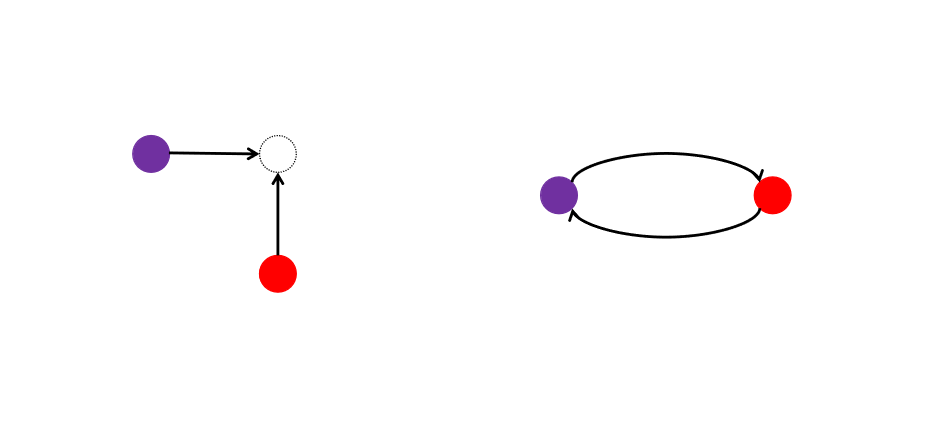
\includegraphics[width=0.6\textwidth, keepaspectratio]{fig2.png}
    \captionsetup{font=footnotesize}
    \caption{根节点中智能体0和智能体1存在路径上的冲突,由此产生了两个约束,通过这两个约束重新生成结点1和结点2}
    \label{figure1}
\end{figure}







\begin{algorithm}
    \renewcommand{\algorithmicrequire}{\textbf{Input:}}
	\renewcommand{\algorithmicensure}{\textbf{Output:}}
    \caption{Get Partial Solution}
    \label{alg:example}
    \begin{algorithmic}[2]
        \REQUIRE 
            game map matrix: $\bf M$,

            a list of all agents' states: $\bf A$
        \ENSURE
            Partial Solution $\bf P$, a two-dimension array of coordinates.

        // definition of Node: 

        // - class attributes: constraints, cost, solution\( may include collisions \)
        
        // - class methods: get first collision, split collision to constraints, 

        \STATE initialize Partial Solution $\bf G$  
        \STATE initialize $open list$
        \STATE initialize $root node$, push it in $open list$
        \WHILE{$open list$ is not empty}
            \STATE get least costly node $n$ from $open list$
            \STATE remove $n$ from $open list$
            \IF {node $n$ has no collision:}
                \STATE then the partial solution has already been founded
            \ELSE
                \STATE get constraints $\bf c$ based on the first collision
                \FOR {constraint $c$ in constraints $\bf c$}
                    \STATE new constriants $\gets$ old constraints of node + $c$
                    \STATE create new node based on new constriants
                    \STATE push new node in $open list$
                \ENDFOR
            \ENDIF
        \ENDWHILE
    \end{algorithmic}
\end{algorithm}


\subsection{CBS的底层寻路——时空联合的A*算法}

\begin{algorithm}
    \renewcommand{\algorithmicrequire}{\textbf{Input:}}
	\renewcommand{\algorithmicensure}{\textbf{Output:}}
    \caption{Space-Time A* Path Finding}
    \label{alg:example}
    \begin{algorithmic}[3]
        \REQUIRE 
            Game map matrix: $\bf M$,

            A single agent: $a$

            A constraints table $\bf c$ 
            
        \ENSURE
            A optimal path of agent $a$

        // definition of Node: (diffrent from Node in CBS algorithm)

        // - class attributes: current position, target, parent node, time, total cost      

        // - class methods: find neighbours, return all avilable position for next time
        

        \STATE initialize $open list$  
        \STATE initialize $closed list$
        \STATE initialize $root node$, push it in $open list$
        \WHILE{$open list$ is not empty}
            \STATE get least costly node $n$ from $open list$
            \STATE remove $n$ from $open list$
            \STATE get $neighbours$  of node
            \FOR{$neighbour$ in $neighbours$}
                \IF{position of $neighbour$ equals target of node}
                    \STATE path $\bf p$ has already been founded
                \ELSE
                    \STATE add $neighbour$ in $open list$
                \ENDIF
            \ENDFOR
        \ENDWHILE
    \end{algorithmic}
\end{algorithm}

\section{实验结果展示}
\section{回顾与展望}

\pagenumbering{arabic}%页码

%分点列举
\begin{itemize}

\item{}

\end{itemize}

实验结果如图\ref{result1}所示

%多排图片,使用时修改textwidth和includegraphics文件名
\begin{figure}[H]
    \centering
    \begin{minipage}[t]{0.3\textwidth}
        \centering
        %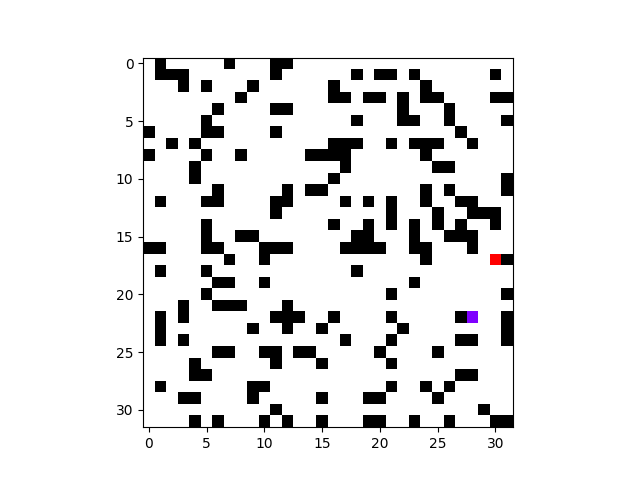
\includegraphics[width=0.5\textwidth]{E:\Azz\CSImproving\MAPF\Report\fig1.png}
        \caption{图}
        \label{result1}
    \end{minipage}
    \begin{minipage}[t]{0.3\textwidth}
        \centering
        %\includegraphics[width=0.7\textwidth]{hongwai2.png}
        \caption{图}
        \label{2}
    \end{minipage}
    \begin{minipage}[t]{0.3\textwidth}
        \centering
        %\includegraphics[width=0.5\textwidth]{hongwai1.png}
        \caption{图}
        \label{3}
    \end{minipage}
\end{figure}


%图片
\begin{figure}[H]
    \centering
    %\includegraphics[width=0.5\textwidth]{hongwai1.png}
    \caption{图}
    \label{4}
\end{figure}

%正式的数学公式
\begin{equation}
    \begin{aligned}
        y=ax+b
    \end{aligned}
    \label{eq1}
\end{equation}

%正式的数学公式(with 大括号)
\begin{equation}
    \begin{cases}
        y=ax+b
    \end{cases}
    \label{eq2}
\end{equation}

%一般数学公式
$$y=ax+b$$

%表格
\begin{table}[H]    
    \begin{spacing}{1.4}  %设置行距
        \centering
        \caption{表}
        %\small  %设置字体
        \begin{tabular}{c|c|c|c}
        %\begin{tabular}{p{2cm}<{\centering}|p{2cm}<{\centering}|p{2cm}<{\centering}|p{2cm}<{\centering}|p{2cm}<{\centering}}  %带有表格宽度控制的表格(少部分表格要用)
            \toprule \\
            \midrule \\
            \hline \\  %表格横线
            \bottomrule
        \end{tabular}
        \label{5}
    \end{spacing}
\end{table}

\end{document}  %结束写文章